\documentclass[11pt]{article}

\usepackage[T1]{fontenc}
\usepackage[utf8]{inputenc}
\usepackage{amsmath,amssymb}
\usepackage{array}
\usepackage{booktabs}
\usepackage{enumitem}
\usepackage{float}
\usepackage{geometry}
\usepackage{graphicx}
\usepackage{hyperref}
\usepackage{tabularx}
\usepackage{xcolor}

\geometry{margin=1in}
\graphicspath{{images/}}
\hypersetup{
  colorlinks=true,
  linkcolor=blue,
  urlcolor=blue
}
\setlist[itemize]{leftmargin=1.4em,itemsep=0.2em,topsep=0.4em}
\setlist[enumerate]{leftmargin=1.6em,itemsep=0.2em,topsep=0.4em}
\let\oldsection\section
\renewcommand{\section}{\clearpage\oldsection}

\newcommand{\missingfigure}[2]{%
  \fbox{%
    \parbox[c][0.22\textheight][c]{0.84\textwidth}{%
      \centering
      Missing figure asset: \texttt{#1}\\[0.5em]
      #2%
    }%
  }%
}

\title{Visibility-Coupled Path Inference in Archaeological Landscapes within LAMP}
\author{}
\date{}

\begin{document}

\maketitle

\section{Personal Details}

\begin{tabularx}{\textwidth}{@{}>{\bfseries}lX@{}}
Name & Ujjwal Singh \\
University & VIT Bhopal University \\
Email & \href{mailto:ujjosing@gmail.com}{ujjosing@gmail.com} \\
LinkedIn & \url{https://www.linkedin.com/in/fallofpheonix} \\
GitHub & \url{https://github.com/fallofpheonix} \\
Country of Residence & India \\
Time Zone & IST (GMT +0530) \\
Primary Language & English \\
Availability & 40+ hours per week during the program period \\
\end{tabularx}

\section{Technical Knowledge}

I have experience building modular, reproducible computational pipelines in Python with a focus on geospatial and simulation-based systems. I am comfortable working with raster data using NumPy- and Rasterio-style workflows, including CRS handling, reprojection, alignment, and nodata management, which are the core requirements for integrating visibility rasters with terrain-driven path inference.

I understand cost-based path modeling, weighted movement surfaces, line-of-sight analysis, and multi-observer viewsheds. I have also worked on controlled parameter calibration and evaluation using metrics such as IoU, F1, recall, and path-density divergence. From a systems perspective, I prioritize deterministic execution, backward compatibility, and configuration-driven workflows so extensions remain debuggable and safe to merge into an existing research codebase.

\section{Abstract}

The Late Antiquity Modeling Project (LAMP) provides deterministic pipelines for archaeological path inference and 3D visibility analysis at the El Bagawat necropolis. While both capabilities exist, the interaction between visibility and movement remains insufficiently validated. The repository already supports visibility-coupled path inference, but its impact on emergent movement patterns and agreement with archaeological evidence has not been systematically evaluated.

This project conducts structured validation and calibration of visibility-coupled path inference within the existing LAMP framework. The work reuses deterministic multi-observer viewshed outputs and integrates them into the path cost model to compare terrain-only and visibility-aware movement scenarios. A controlled evaluation pipeline measures how visibility changes path distributions using IoU, F1 score, top-k recall, and path-density divergence. In parallel, the project performs sensitivity analysis over the visibility weight parameter to identify stable operating regimes.

The expected outcome is a reproducible evaluation framework that establishes whether visibility acts as a meaningful constraint on movement in archaeological landscapes. Even if visibility does not improve agreement with archaeological evidence, the project still delivers a validated coupling interface, calibrated parameter ranges, and comparison artifacts that support later archaeological interpretation.

\section{Problem Statement}

\subsection{Existing LAMP Capabilities}

The LAMP repository implements two core deterministic geospatial pipelines for the El Bagawat necropolis:

\begin{itemize}
  \item \textbf{Task 1} performs probabilistic path tracing using a multi-factor cost surface derived from slope, roughness, surface conditions, and path priors. Outputs include movement-cost rasters, path density maps, and vectorized predicted pathways.
  \item \textbf{Task 2} computes multi-observer visibility through line-of-sight analysis over terrain and building geometry, aggregating per-observer viewsheds into a continuous visibility probability raster.
\end{itemize}

The pipelines are modular and CLI-driven, with a shared configuration system and file-based artifact exchange. Task 2 exports \texttt{viewshed\_probability.tif}, and Task 1 already supports an extended cost model with an optional visibility term. Comparison mode is also available, allowing baseline and visibility-coupled runs within one execution.

\subsection{Limitations of the Current Pipeline}

The codebase contains visibility coupling, but not a rigorous validation layer. Current verification is limited to smoke tests and synthetic scenarios. Real end-to-end integration between Task 2 outputs and Task 1 inputs has not been fully exercised under production conditions due to environmental constraints such as GDAL binding issues.

The repository also lacks systematic evaluation against archaeological ground truth. Default configurations do not include known-path labels, so metrics such as IoU, F1 score, and top-k recall cannot yet be computed against real evidence. Sensitivity analysis of the visibility weight is also incomplete, which means the system does not currently quantify whether visibility materially improves path inference or simply perturbs it.

\subsection{Identified Gap}

The gap is not missing implementation; it is missing characterization. Visibility and movement are already connected in code, but effectively decoupled at the level of scientific interpretation. The current pipeline does not yet answer:

\begin{enumerate}
  \item Whether visibility-aware cost functions align more closely with archaeological evidence.
  \item How sensitive inferred paths are to the visibility weight parameter.
  \item Where visibility redistributes movement probability across the landscape.
\end{enumerate}

This project closes that gap by converting visibility coupling from an implemented feature into a calibrated and testable research component.

\section{System Design}

\subsection{System Overview}

The proposed system adds an evaluation and calibration layer over the existing LAMP implementation. It does not replace core modules. Instead, it orchestrates Task 1 and Task 2 into a controlled experimental workflow with two execution modes:

\begin{itemize}
  \item \textbf{Baseline mode:} terrain-, surface-, and prior-driven path inference only.
  \item \textbf{Coupled mode:} identical execution with an additional visibility-derived penalty term.
\end{itemize}

Both modes run under identical conditions and are compared through shared outputs and metrics.

\begin{figure}[H]
\centering
\IfFileExists{images/pipeline.png}{%
  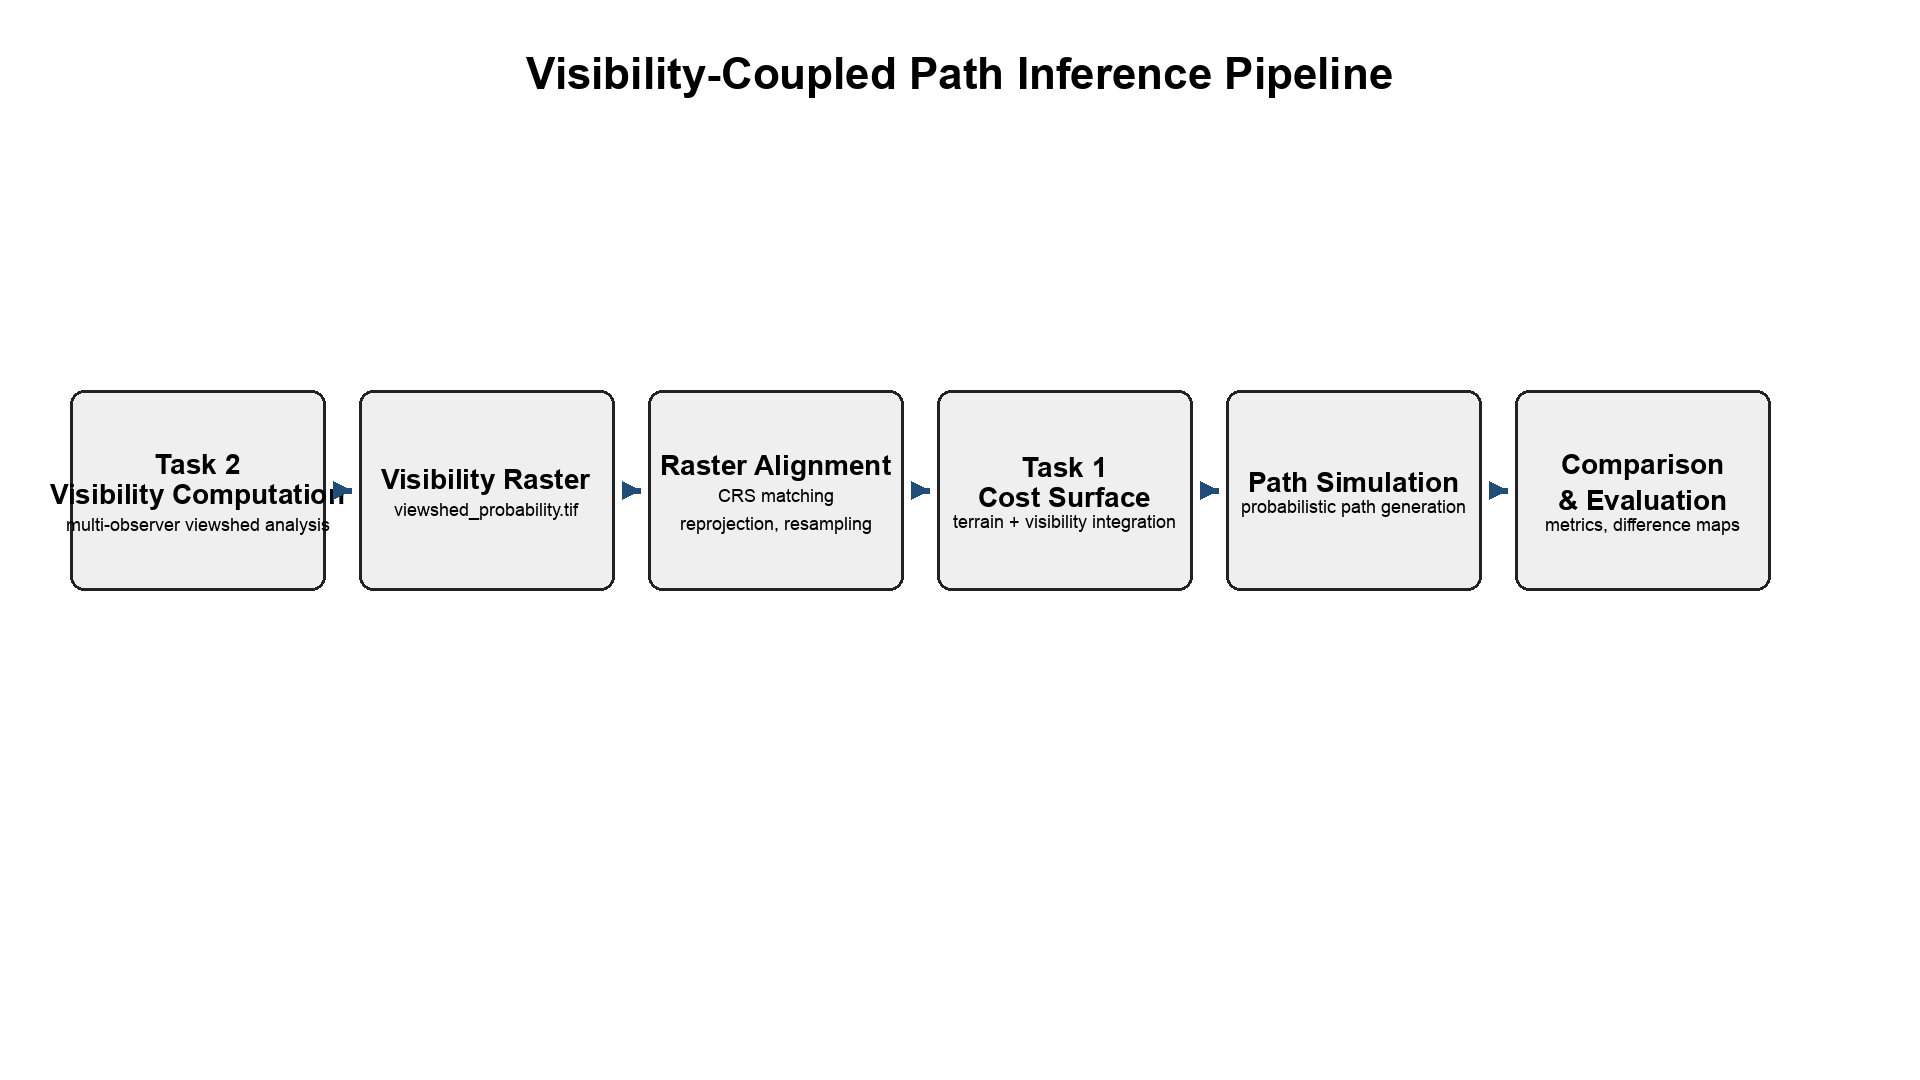
\includegraphics[width=\textwidth]{pipeline.png}%
}{%
  \missingfigure{images/pipeline.png}{Insert the publication-quality pipeline diagram.}%
}
\caption{End-to-end visibility-coupled path inference pipeline.}
\label{fig:system-pipeline}
\end{figure}

\subsection{Core Components}

\begin{enumerate}
  \item \textbf{Visibility Generator (Task 2):} Produces \texttt{viewshed\_probability.tif} from multi-observer line-of-sight analysis.
  \item \textbf{Raster Alignment Layer:} Ensures compatibility between the Task 2 visibility raster and the Task 1 DEM grid by validating CRS, transform, and shape, then reprojecting when required.
  \item \textbf{Cost Surface Engine (Task 1 extension):} Builds movement cost from terrain factors plus an optional visibility term.
  \item \textbf{Path Simulation Engine:} Performs probabilistic path sampling over the computed cost surface.
  \item \textbf{Calibration Module:} Searches over visibility weights under explicit constraints.
  \item \textbf{Comparison and Evaluation Layer:} Generates paired outputs, summary metrics, and density redistribution artifacts.
\end{enumerate}

\subsection{Visibility-Coupled Cost Model}

The movement model uses the following deterministic cost formulation:

\[
C = w_s S + w_r R + w_t T + w_p (1 - P) + w_v (1 - V)
\]

where:

\begin{itemize}
  \item $S$ is normalized slope.
  \item $R$ is normalized roughness.
  \item $T$ is normalized surface penalty.
  \item $P$ is path prior probability.
  \item $V$ is visibility probability.
\end{itemize}

Model invariants:

\begin{itemize}
  \item $\sum w = 1$.
  \item $w_v = 0$ reduces exactly to the baseline pipeline.
  \item Nodata and obstacle cells retain infinite cost.
  \item Visibility acts as a cost modifier, not as an independent path generator.
\end{itemize}

\begin{figure}[H]
\centering
\IfFileExists{images/cost.png}{%
  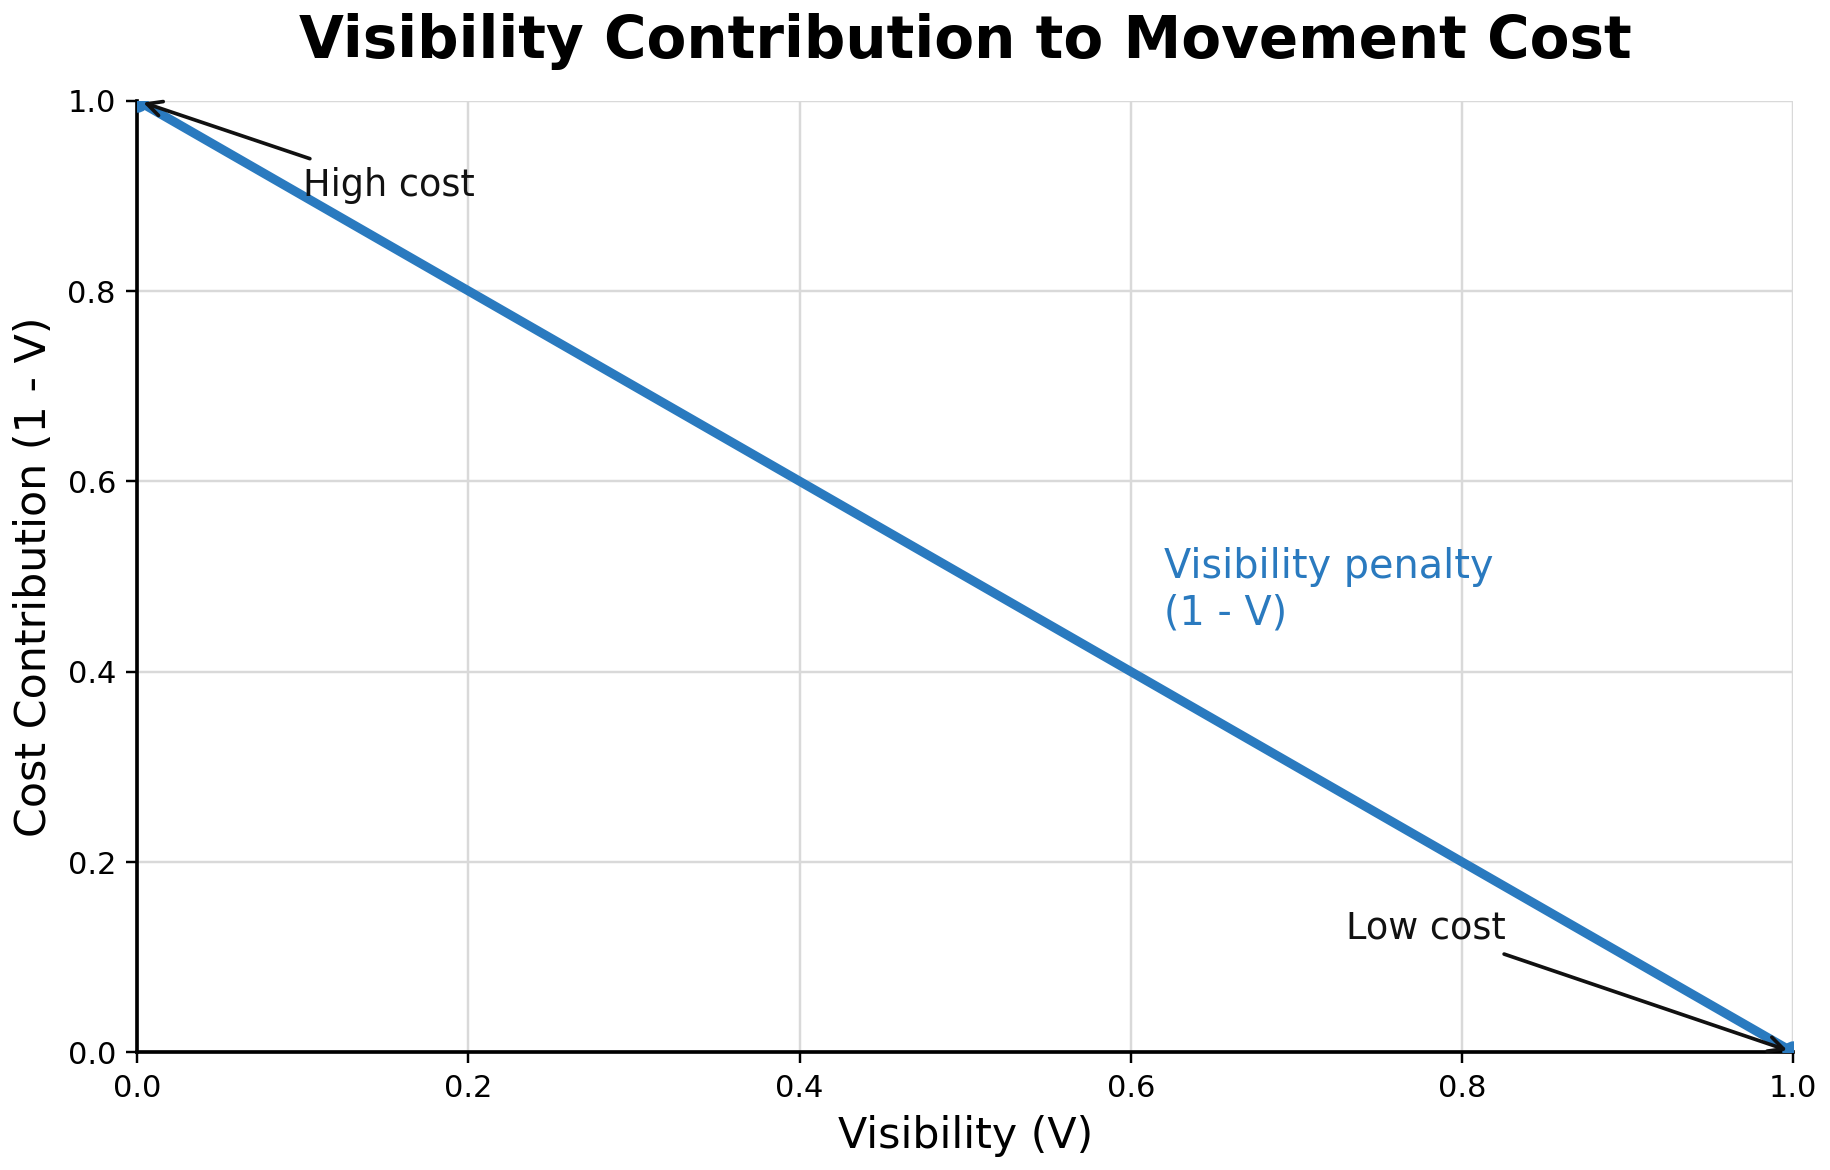
\includegraphics[width=0.7\textwidth]{cost.png}%
}{%
  \missingfigure{images/cost.png}{Insert the visibility contribution plot.}%
}
\caption{Visibility contribution to the movement cost function.}
\label{fig:cost-effect}
\end{figure}

\subsection{Data Flow and Execution}

The coupling interface is raster-based and deterministic:

\begin{verbatim}
Task 2 inputs -> viewshed_probability.tif -> alignment to Task 1 DEM grid
-> cost surface construction -> path simulation -> comparison -> metrics
\end{verbatim}

Task 1 consumes visibility through additive CLI arguments:

\begin{verbatim}
--visibility-raster <path>
--w-visibility <value>
--compare-visibility-coupling
\end{verbatim}

\begin{figure}[H]
\centering
\IfFileExists{images/dataflow.png}{%
  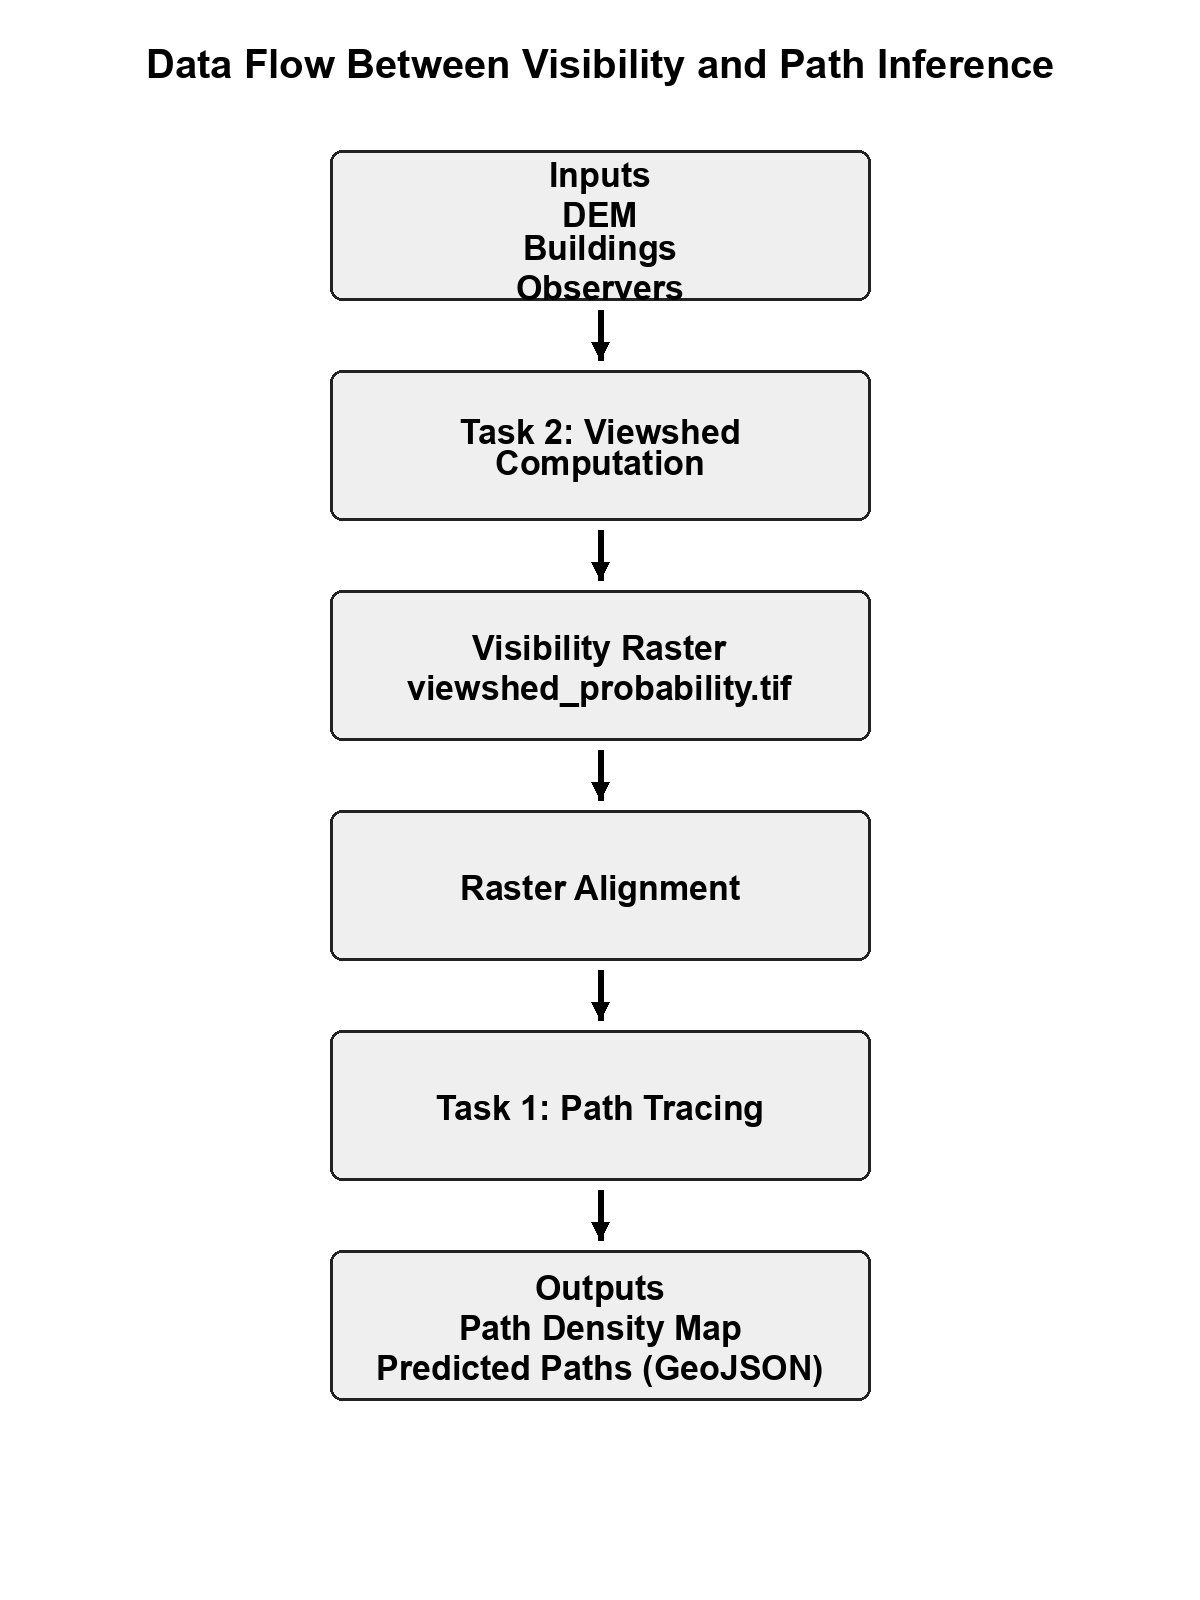
\includegraphics[width=\textwidth]{dataflow.png}%
}{%
  \missingfigure{images/dataflow.png}{Insert the vertical Task 2 to Task 1 data flow diagram.}%
}
\caption{Data flow between visibility computation and path inference.}
\label{fig:path-sampling-flow}
\end{figure}

\subsection{Technology Stack and Constraints}

\begin{itemize}
  \item \textbf{Core environment:} Python, NumPy-style numerical workflows, Rasterio, GeoPandas, Shapely.
  \item \textbf{Primary modules:} \texttt{src/lamp/tasks/path\_tracing/}, \texttt{src/lamp/tasks/viewsheds/}, and \texttt{src/lamp/api/cli.py}.
  \item \textbf{Execution scripts:} \texttt{scripts/run\_path\_tracing.py} and \texttt{scripts/run\_viewsheds.py}.
  \item \textbf{Constraints:} CPU-only execution, local environment, optional GDAL dependency for Task 2 runtime.
\end{itemize}

\section{Implementation Plan}

\subsection{Stepwise Development Plan}

\begin{enumerate}
  \item \textbf{Environment stabilization and baseline verification.} Ensure Task 1 and Task 2 run end-to-end, verify baseline outputs, and confirm that comparison-mode smoke tests behave deterministically.
  \item \textbf{Task 2 execution enablement.} Resolve GDAL or \texttt{osgeo} issues and generate a real \texttt{viewshed\_probability.tif} from the El Bagawat dataset.
  \item \textbf{Raster alignment and coupling verification.} Align the visibility raster to the Task 1 DEM grid, clip values into $[0,1]$, and validate the coupled path run on real data.
  \item \textbf{Baseline vs. coupled execution.} Run both modes under identical inputs and store paired outputs such as \texttt{baseline/}, \texttt{visibility\_coupled/}, \texttt{comparison\_density\_delta.tif}, and \texttt{comparison\_summary.json}.
  \item \textbf{Calibration and sensitivity analysis.} Sweep $w_v$ over a bounded range such as $\{0.0, 0.1, 0.2, 0.3, 0.4\}$ while renormalizing the remaining weights.
  \item \textbf{Evaluation.} Compute label-based metrics when known paths are available; otherwise compute density divergence and redistribution patterns.
  \item \textbf{Artifact generation and reporting.} Export publication-quality figures, GIS layers, tables, and reproducibility notes.
\end{enumerate}

\section{Integration with the Existing LAMP Codebase}

\subsection{Target Modules and Files}

\begin{itemize}
  \item \texttt{scripts/run\_path\_tracing.py}: primary Task 1 orchestration entry point.
  \item \texttt{scripts/run\_viewsheds.py}: Task 2 visibility raster generation.
  \item \texttt{src/lamp/tasks/path\_tracing/simulation/cost\_surface.py}: visibility-aware cost construction.
  \item \texttt{src/lamp/tasks/path\_tracing/simulation/calibration.py}: weight tuning and evaluation.
  \item \texttt{src/lamp/tasks/path\_tracing/config.py}: visibility parameters and raster-path configuration.
  \item \texttt{src/lamp/tasks/viewsheds/visibility.py}: multi-observer visibility aggregation.
  \item \texttt{src/lamp/config/pipeline.yaml}: centralized configuration for \texttt{visibility\_raster}, \texttt{w\_visibility}, and comparison mode.
\end{itemize}

\subsection{Task 1 / Task 2 Data Interface}

The coupling contract is intentionally narrow:

\begin{itemize}
  \item \textbf{Producer:} Task 2 writes \texttt{viewshed\_probability.tif}.
  \item \textbf{Consumer:} Task 1 reads the aligned raster and inserts $(1-V)$ into the cost surface.
  \item \textbf{Reference grid:} the Task 1 DEM defines CRS, transform, resolution, and raster dimensions.
\end{itemize}

Alignment checks are explicit:

\begin{itemize}
  \item CRS equality
  \item transform equality
  \item width and height equality
  \item reprojection with bilinear resampling when mismatch exists
  \item nodata conversion to NaN before clipping to $[0,1]$
\end{itemize}

\subsection{Backward Compatibility Strategy}

No existing workflows should break. The coupling remains opt-in and parameter-controlled:

\begin{itemize}
  \item If \texttt{w\_visibility = 0} or no visibility raster is provided, Task 1 must behave exactly like the original baseline.
  \item Existing arguments remain valid; visibility-related arguments are additive.
  \item Standard outputs remain unchanged. Comparison artifacts appear only in comparison mode.
\end{itemize}

\section{Timeline}

\subsection{Community Bonding Period (Weeks 0--1)}

\begin{itemize}
  \item \textbf{Week 0:} Deep dive into Task 1 and Task 2 internals, verify prototype assumptions against repository structure, and identify integration gaps.
  \item \textbf{Week 1:} Stabilize the local environment, resolve GDAL issues, and finalize the evaluation plan with mentors.
\end{itemize}

\subsection{Coding Phase I (Weeks 2--6)}

\begin{itemize}
  \item \textbf{Week 2:} Reproduce Task 1 baseline on the El Bagawat dataset.
  \item \textbf{Week 3:} Execute Task 2 and generate the visibility raster.
  \item \textbf{Week 4:} Implement and verify raster alignment.
  \item \textbf{Week 5:} Run baseline and coupled scenarios under shared inputs.
  \item \textbf{Week 6:} Fix edge cases related to nodata, misalignment, and scale.
\end{itemize}

\subsection{Coding Phase II (Weeks 7--11)}

\begin{itemize}
  \item \textbf{Week 7:} Implement the bounded calibration loop over visibility weights.
  \item \textbf{Week 8:} Collect outputs and prepare derived maps.
  \item \textbf{Week 9:} Compute label-based or distribution-based evaluation metrics.
  \item \textbf{Week 10:} Perform sensitivity analysis and identify stable operating regimes.
  \item \textbf{Week 11:} Generate final figures, metric tables, and GIS artifacts.
\end{itemize}

\subsection{Final Week (Week 12)}

\begin{itemize}
  \item Write the reproducibility guide and CLI usage notes.
  \item Finalize configuration files and respond to mentor feedback.
  \item Prepare the final submission report and supporting artifacts.
\end{itemize}

\section{Deliverables}

\begin{itemize}
  \item End-to-end Task 2 to Task 1 coupling on real data.
  \item Validated visibility raster integration into the path-tracing pipeline.
  \item Comparison-mode execution producing baseline and visibility-coupled outputs.
  \item Calibration runs over bounded visibility weights.
  \item GIS artifacts including density rasters, delta maps, and predicted pathway vectors.
  \item Reproducibility documentation covering CLI commands, configuration, and output interpretation.
\end{itemize}

\section{Evaluation Plan}

\subsection{Baseline vs. Visibility-Coupled Comparison}

Two configurations are executed under identical inputs:

\begin{itemize}
  \item \textbf{Baseline:} $w_v = 0$.
  \item \textbf{Coupled:} $w_v > 0$ with all other variables held constant apart from renormalization.
\end{itemize}

The comparison evaluates path density maps, predicted paths, and spatial redistribution of movement probability. Current repository smoke-test outputs already demonstrate that the comparison pipeline emits usable paired artifacts, but those figures should be replaced with real-data results before final submission.

\begin{figure}[H]
\centering
\IfFileExists{images/comparison.png}{%
  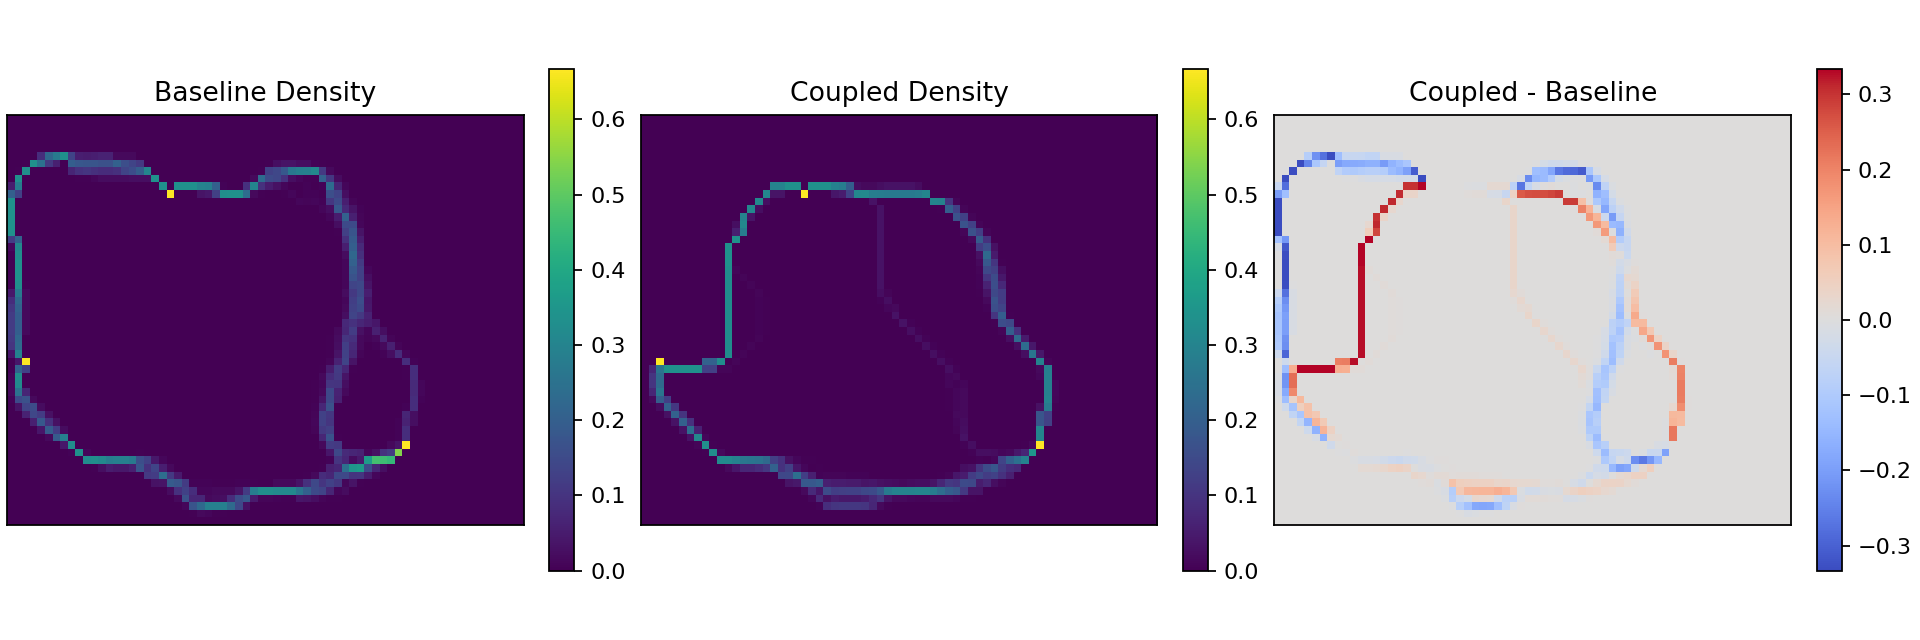
\includegraphics[width=\textwidth]{comparison.png}%
}{%
  \missingfigure{images/comparison.png}{Insert side-by-side baseline and visibility-coupled path density maps.}%
}
\caption{Comparison of baseline and visibility-coupled path density distributions.}
\label{fig:comparison}
\end{figure}

\subsection{Metrics with Ground Truth}

If known archaeological paths are available, evaluation uses:

\begin{itemize}
  \item IoU for spatial overlap.
  \item F1 score for balance between precision and recall.
  \item Top-k recall for whether the highest-probability predicted paths intersect known routes.
\end{itemize}

\subsection{Fallback without Ground Truth}

If labels are unavailable, the evaluation falls back to distributional analysis:

\begin{itemize}
  \item path-density divergence
  \item density delta mapping
  \item spatial redistribution analysis relative to high-visibility and low-visibility zones
\end{itemize}

When reference paths are available, a standalone residual heatmap is useful for localizing overprediction and underprediction. If no labels exist, the same slot can instead show the coupled-minus-baseline redistribution map.

\begin{figure}[H]
\centering
\IfFileExists{images/difference.png}{%
  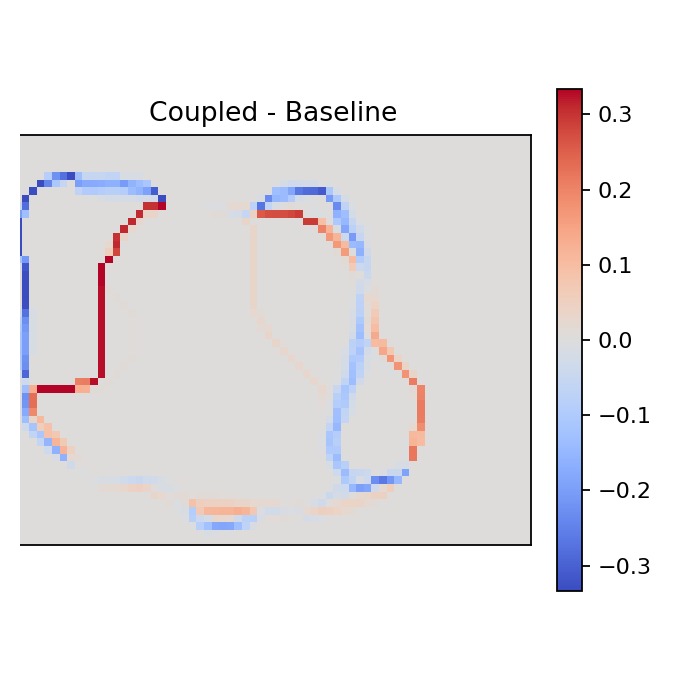
\includegraphics[width=\textwidth]{difference.png}%
}{%
  \missingfigure{images/difference.png}{Insert the red-white-blue difference heatmap for movement redistribution.}%
}
\caption{Spatial redistribution of movement probability.}
\label{fig:density-difference}
\end{figure}

\subsection{Sensitivity Analysis}

Sensitivity analysis measures how path structure changes as $w_v$ increases. The objective is not only accuracy improvement, but stability analysis: whether visibility produces a consistent shift or overwhelms the terrain model.

\begin{figure}[H]
\centering
\IfFileExists{images/sensitivity.png}{%
  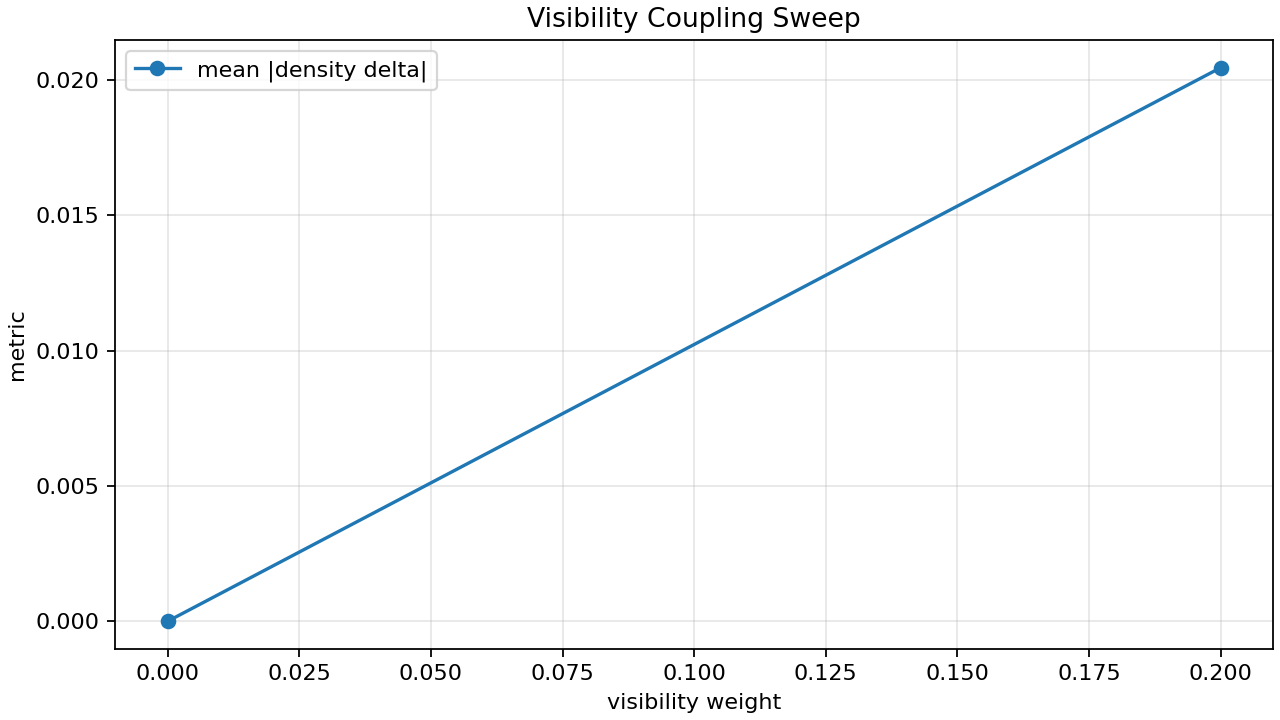
\includegraphics[width=0.78\textwidth]{sensitivity.png}%
}{%
  \missingfigure{images/sensitivity.png}{Insert the visibility-weight sensitivity plot.}%
}
\caption{Sensitivity of the path-density response to the visibility weight.}
\label{fig:sensitivity}
\end{figure}

\section{Risks and Mitigation}

\begin{itemize}
  \item \textbf{Task 2 execution failure due to GDAL or \texttt{osgeo} issues.} Mitigate during Weeks 0--2; fallback to precomputed or synthetic visibility only for development smoke tests.
  \item \textbf{Raster misalignment.} Enforce CRS, transform, and shape checks before coupling and validate alignment with dedicated test cases.
  \item \textbf{No ground truth data.} Shift evaluation emphasis to density divergence and redistribution analysis; report results as exploratory when necessary.
  \item \textbf{Visibility has no measurable impact.} Treat as a valid scientific result and still deliver the calibration and negative-result framework.
  \item \textbf{Overfitting to the visibility weight.} Restrict the search range and report stable operating regions rather than a single tuned value.
\end{itemize}

\section{Why This Project}

This proposal aligns directly with LAMP's objective of reconstructing embodied spatial experience in archaeological landscapes. The repository already contains both the movement and visibility pipelines. What it lacks is a controlled mechanism for proving whether their coupling is scientifically useful. This project addresses exactly that layer without introducing architectural churn.

The contribution is intentionally conservative from an engineering perspective: reuse current modules, preserve CLI contracts, keep coupling optional, and treat reproducibility as a first-class deliverable. That keeps scope bounded and makes the outcome immediately usable by the LAMP research team.

\section{References}

\begin{enumerate}
  \item Perez-Garcia, J. L., Mozas-Calvache, A. T., Gomez-Lopez, J. M., and Jimenez-Serrano, A. Modelling the evolution of the archaeological works developed in Qubbet el-Hawa (Aswan, Egypt). \textit{International Archives of the Photogrammetry, Remote Sensing and Spatial Information Sciences}, 2021.
  \item Wrozynski, R., et al. 3D visibility analysis workflows in GIS and game-engine environments, 2024.
  \item Kiourt, C., et al. Agent-based and terrain-aware mobility modeling in archaeological landscapes, 2026.
  \item Jaturapitpornchai, R., et al. LiDAR segmentation and model sensitivity in archaeological reconstruction, 2024.
  \item QGIS Visibility Analysis Plugin Documentation.
\end{enumerate}

\end{document}
